\documentclass[../../main.tex]{subfiles}
\begin{document}

{\bf [解答]}

\begin{figure}[htb]
  \centering
  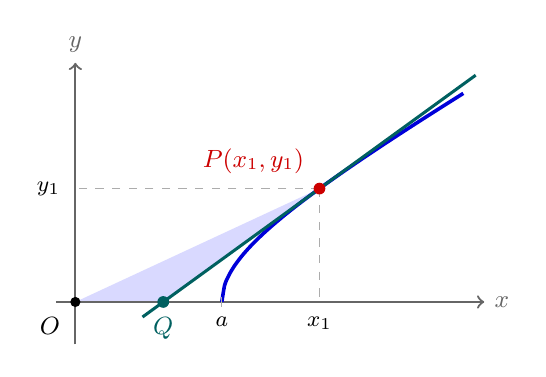
\begin{tikzpicture}[x=1.55cm, y=1.35cm,
    every node/.style={font=\small}]
    % a=6/5, b=4/5, P=(2,16/15), Q=(18/25,0).
    \coordinate (O) at (0,0);
    \coordinate (Q) at (0.72,0);
    \coordinate (P) at (2,1.066667);
    \fill[blue!15] (O)--(Q)--(P)--cycle;
    \draw[->, thick, gray!80!black] (-0.16,0)--(3.35,0)
    node[right] {$x$};
    \draw[->, thick, gray!80!black] (0,-0.4)--(0,2.25)
    node[above] {$y$};
    \draw[line width=1.3pt, blue!85!black,
    domain=1.2:3.18, samples=90, smooth]
    plot (\x,{2/3*sqrt(max(\x*\x-1.44,0))});
    \draw[line width=1.1pt, teal!75!black] (0.55,-0.141667)
    -- (3.28,2.133333);
    \draw[dashed, gray!65] (P)--(2,0) (P)--(0,1.066667);
    \draw[thin, gray!65] (1.2,0.05)--(1.2,-0.05);
    \node[circle, fill, inner sep=1.3pt] at (O) {}; \node[below left=2pt] at (O) {$O$};
    \node[circle, fill=red!80!black, inner sep=1.5pt] at (P) {}; \node[red!80!black, above left=2pt] at (P) {$P(x_1,y_1)$};
    \node[circle, fill=teal!75!black, inner sep=1.5pt] at (Q) {}; \node[teal!75!black, below=2pt] at (Q) {$Q$};
    \node[below=2pt, font=\footnotesize] at (1.2,0) {$a$};
    \node[below=2pt, font=\footnotesize] at (2,0) {$x_1$};
    \node[left=2pt, font=\footnotesize] at (0,1.066667) {$y_1$};
  \end{tikzpicture}
  \caption{双曲線上の点 $P$ における接線と $x$ 軸との交点 $Q$}
  \label{fig:1967_3_tangent_triangle}
\end{figure}

与えられた双曲線
\begin{align}
  \dfrac{x^2}{a^2} - \dfrac{y^2}{b^2} = 1
\end{align}
について考える．
点 $P(x_1,y_1)$ での接線は $\dfrac{x_1}{a^2}x - \dfrac{y_1}{b^2}y = 1$ だから，
これと$x$軸との交点は $Q\left(\dfrac{a^2}{x_1}, 0\right)$ である．

\paragraph{(1)}

まず $\dfrac{y_1^2}{b^2} = \dfrac{x_1^2}{a^2} - 1$ 及び $y_1, b > 0$ から
\begin{align}
  y_1 = b \sqrt{\dfrac{x_1^2}{a^2} - 1}
\end{align}
である．従って$\triangle OPQ$の面積は，$P$から$x$軸におろした垂足$P'(x_1,0)$として
\begin{align}
  \triangle OPQ
  = \dfrac{1}{2}|OQ||PP'|
  = \dfrac{1}{2}\dfrac{a^2}{x_1}y_1
  = \dfrac{1}{2} \dfrac{a^2}{x_1} b \sqrt{\dfrac{x_1^2}{a^2} - 1} \label{eq:1}
\end{align}
である．

\paragraph{(2)}

\cref{eq:1}より求める極限値は
\begin{align}
  \triangle OPQ
  &= \dfrac{ab}{2} \sqrt{\dfrac{x_1^2 - a^2}{x_1^2}} \\
  &= \dfrac{ab}{2} \sqrt{1 - a^2 / x_1^2}
  \xrightarrow{x_1 \to \infty} \dfrac{ab}{2}
\end{align}
である．

\newpage

\end{document}
